\documentclass[12pt,a4paper]{article}

\usepackage[utf8]{inputenc}
\usepackage[IL2]{fontenc}
\usepackage{mathtools}
\usepackage{gensymb}
\usepackage{siunitx}
\usepackage[czech]{babel}
\usepackage{graphicx}
\usepackage{amsmath}
\usepackage{cleveref}
\usepackage{xcolor}
\usepackage{listings}

\definecolor{mGreen}{rgb}{0,0.6,0}
\definecolor{mGray}{rgb}{0.5,0.5,0.5}
\definecolor{mPurple}{rgb}{0.58,0,0.82}
\definecolor{backgroundColour}{rgb}{0.95,0.95,0.92}

\lstdefinestyle{CStyle}{
	backgroundcolor=\color{backgroundColour},   
	commentstyle=\color{mGreen},
	keywordstyle=\color{magenta},
	numberstyle=\tiny\color{mGray},
	stringstyle=\color{mPurple},
	basicstyle=\footnotesize,
	breakatwhitespace=false,         
	breaklines=true,                 
	captionpos=b,                    
	keepspaces=true,                 
	numbers=left,                    
	numbersep=5pt,                  
	showspaces=false,                
	showstringspaces=false,
	showtabs=false,                  
	tabsize=2,
	language=C
}

\topmargin = -15mm
\textwidth=150mm
\textheight=240mm

\begin{document}
	\begin{titlepage}
		\begin{center}
			%%\includegraphics[width=1\textwidth]{SEM LOGO}
			\vspace{5cm}
			
			\Huge
			\textbf{Vestavvěné systémy}
			
			\vspace{0.5cm}
			\LARGE
			Semestrální práce
			
			\vspace{1.5cm}
			\begin{figure}[h]
				\centering
				
\includegraphics[height=8cm]{logo}

			\end{figure}
			
			\vfill
			
			
			\vspace{0.8cm}			
			
		\end{center}
		\begin{flushleft}
			Vypracovali:\\ 
			\hspace{1cm}Vlk Jan \\
			\hspace{1cm}Hazdra Martin \\
			
			Cvičící: Ing. Zdeněk Novák Ph.D.\\
			Ročník: 1\\
			Skupina: L4\\
			
		\end{flushleft}
	\end{titlepage}
	

\newpage

\section*{Zadání}
Zadání č. 2:\\
Sestavte program pro dvoupolohový regulátor pro regulaci otáček stejnosměrného motoru. Signál skutečné hodnoty otáček se snímá pulzním čidlem, žádaná hodnota otáček se zadává pomocí potenciometru. Jsou-li žádané otáčky vyšší než skutečné, spíná se hlavní tranzistor pulzního měniče, jsou-li žádané otáčky menší než skutečné, hlavní tranzistor se vypíná.


\newpage
\section*{Řešení}
\subsection*{Deklarace proměnných}
\begin{lstlisting}[style=CStyle]
	//Vysledek adc konverze - potenciometr
	uint32_t potResult = 0;
	
	//Hodnota casovace
	uint32_t uSClock = 0;
	
	//Hodnota casovace na posledni hrane enkoderu
	uint32_t uSlastPulseTime = 0;
	
	//Hodnota casovace na aktualni hrane enkoderu
	uint32_t uStimeNow = 0;
	
	//Rozdil hodnot casovace mezi hranami
	uint32_t uStimeDelta = 108882172;
	
	//Posledni stav senzoru
	uint8_t lastPinState = 1;
	uint8_t currentPinState = 0;
	
	//Prepocitana hodnota z potenciometru na ocekavanou periodu
	uint32_t requestedSpeed = 0;
\end{lstlisting}
\subsection*{Nastavení převodníku a časovače}
\begin{lstlisting}[style=CStyle]
	//Nastaveni automatickeho zapisovani stavu potenciomteru do pameti
	HAL_ADC_Start_DMA(&hadc3, &potResult, 1);
	//Zapnuti casovace - mereni v mikrosekundach
	HAL_TIM_Base_Start(&htim2);

\end{lstlisting}
\subsection*{Hlavní smyčka programu}
\begin{lstlisting}[style=CStyle]
	while (1)
	{
		//precteni hodnoty casovace
		uSClock = __HAL_TIM_GET_COUNTER(&htim2);
		
		//Vyhodnoceni regulatoru
		if(requestedSpeed<uStimeDelta){
			//Motor se toci pomaleji nez je nastaveno
			HAL_GPIO_WritePin(HSS_Pin_GPIO_Port, HSS_Pin_Pin, 1);
			HAL_GPIO_WritePin(LSS_Pin_GPIO_Port, LSS_Pin_Pin, 1);
			
		}
		if(requestedSpeed>uStimeDelta){
			//Motor se toci rychleji nez je nastaveno
			HAL_GPIO_WritePin(HSS_Pin_GPIO_Port, HSS_Pin_Pin, 0);
			HAL_GPIO_WritePin(LSS_Pin_GPIO_Port, LSS_Pin_Pin, 0);
			
		}
		//precteni stavu senzoru polohy
		currentPinState = HAL_GPIO_ReadPin(RPM1_GPIO_Port, RPM1_Pin);
		//Nastaveni casu v aktualnim cyklu
		uStimeNow=uSClock;
		if(currentPinState == 1 && lastPinState == 0){
			// Detekovana hrana
			//Ulozeni stavu senzoru
			lastPinState = 1;
			//Ulozeni casu posledni hrany
			uSlastPulseTime = uStimeNow;
			
		}
		if(currentPinState == 0){
			//Resetovani stavu senzoru
			lastPinState = 0;
		}
		
		//Vyhodnoceni rychlosti otaceni
		uStimeDelta=uStimeNow-uSlastPulseTime;
\end{lstlisting}
\subsection*{Čtení hodnoty z potenciometru}
\begin{lstlisting}[style=CStyle]
	void HAL_ADC_ConvCpltCallback(ADC_HandleTypeDef* hadc){
		//Konverze dokoncena, ulozeni hodnot a nastaveni vyzadovanych otacek
		potResult = HAL_ADC_GetValue(hadc);
		requestedSpeed = potResult*2;
	}
\end{lstlisting}
\subsection*{Zapojení}
\begin{figure}[h]
	\centering
	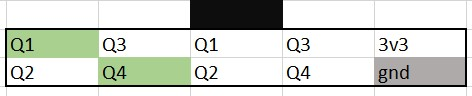
\includegraphics[height=1.5cm]{pins}
	\caption{Rozložení pinů na H-můstku}
	\label{pins}
\end{figure}
\begin{figure}[h]
	\centering
	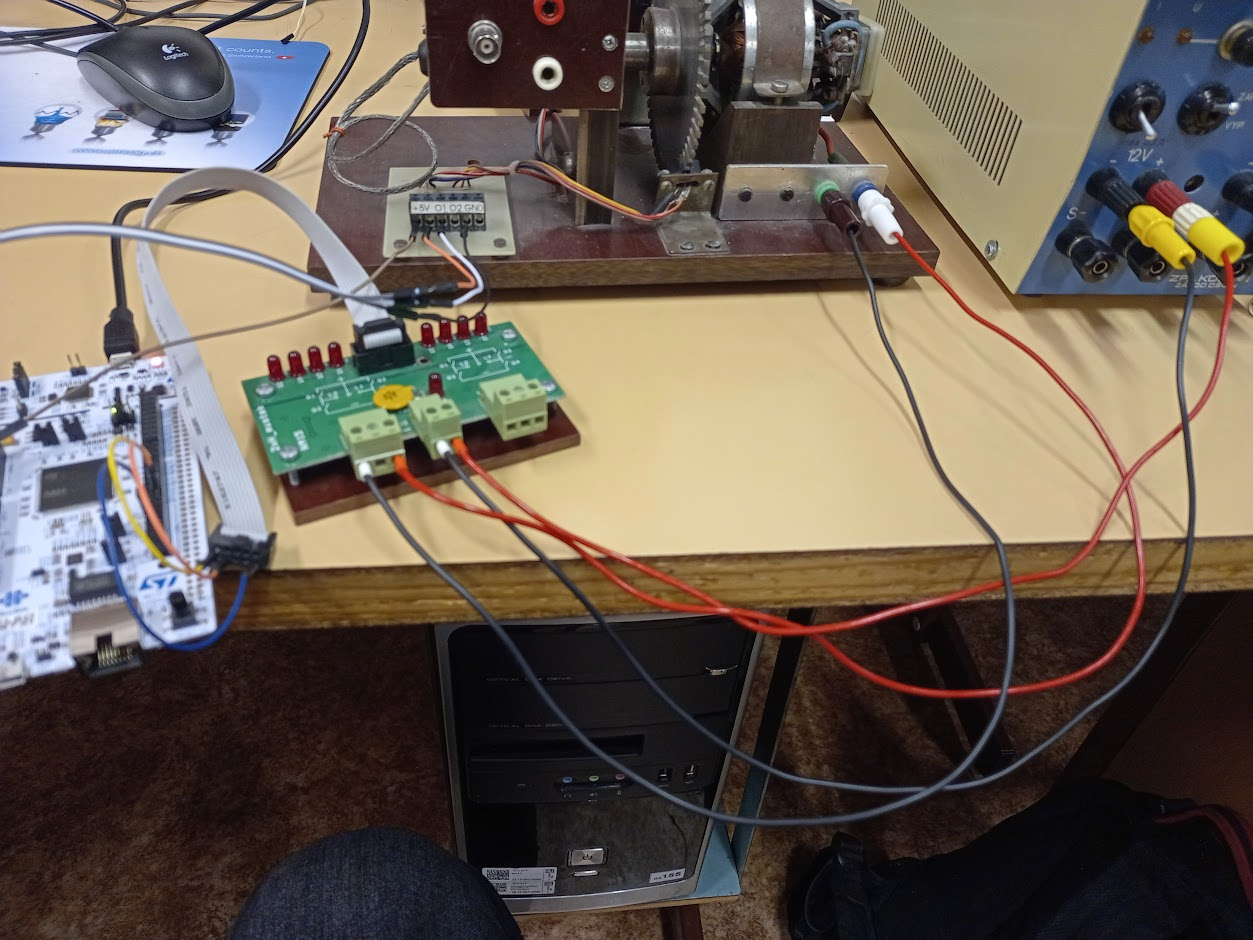
\includegraphics[height=10cm]{zapojeni}
	\caption{Zapojení obvodu}
	\label{zapoj}
\end{figure}

\newpage
\section{Závěr}
Naším úkolem bylo vytvořit dvoupolohové řízení otáček stejnosměrného motoru. Žádanou hodnotu otáček jsme zadávali pomocí potenciometru připojeného na ADC převodník a skutečnou hodnotu otáček jsme zjišťovali pomocí pulzního čidla a časovače vestavěného v procesoru. Problémem tohoto způsobu řízení byla nemožnost nastavit potenciometr na nulu, tedy zastavit motor úplně.




\end{document}
